\documentclass{article}

\usepackage{graphicx}
\usepackage{hyperref}
  \title{Personal Development Report(Evaluation 1)}
  \author{Danil Burov}
  \date{\today}

\begin{document}

\maketitle
\newpage
\tableofcontents
\newpage

\section{Introduction}
My name is Danil Burov and I am studying Information Technology in Fontys, Venlo. I am specializing in 
Embedded Software back in Venlo and the reason I chose this minor is because I think that AI is a very 
ongoing topic and I wanted to get more familiar with it. Especially because I think that AI has a big 
implication when it comes down to IoT devices.

\section{Learning outcome 1 - Societal impact}
\underline{\textbf{In my own words:}}\\
Able to analyze societal impact of a project\\\\
  %Try summarizing the learning outcome with one sentece
\underline{\textbf{Explanation:}}\\
Societal impact is one of the most important contextual parts of the project. Every time a person 
starts a project an evaluation on the societal impact should be done in order to understand 'Why?'
a project is being done on the given topic.
  %Describe the learning outcome how you understand it
\subsection{First evaluation}
During the first weeks of the minor I had the opportunity to think about the societal impact of the projects I will 
be working on. Since the beginning I had an idea of what my personal project could look like. However, I was not that aware
what could be the societal impact of my project. With the help of the technical coach 'Jacco'.\\\\
To see the feedpulse checkpoint regarding this evaluation go to Figure \ref{fig:appendix_image1}.
\\\\
\underline{\textbf{Self assesment: Orientating}}

\section{Learning outcome 2 - Investigative problem solving}
\underline{\textbf{In my own words:}}\\
Critically analyze the recongnize and solve problems.\\\\ 
\underline{\textbf{Explanation:}}\\
From this learning outcome I will further develop my investigative and problem solving skills regarding 
how AI is used in the project, is it doing as intended and if not how to approach the problem and solve it 
eventually.

\subsection{First evaluation}
During the first weeks I had to tackle several problems. In the beginnig the course was presented with some stakeholders 
who presented to us what issues they have with their companies and what they would like to add to their business. I was given 
the opportunity to think of an idea that solves a business case and so I created a project proposal for one of the companies that visited us. 
The proposal is based on the problem that the company has.\\\\
%The link is not working
To see the full proposal go to this link: \href{https://github.com/BurovDanil/MinorAI/blob/main/Documents/Project%20Proposal/Proposal.md}{project proposal}\\\\
  \underline{\textbf{Self assesment: Orientating}}
%Upload the project proposal
%During the first weeks I already had to deal with investagative problem solving. In my personal project I had to deal 
%with the legal aspect of my project. In order to solve the issue I went to talk to one of the legal consultants about 
%how I could tackle the problem. In the end of the discussion we managed to resolve the problem with writing a small 'Disclaimer' 
%for the intended usage of the AI model that will be created. As well as during my first stakeholder meeting with my group we were presented
%with an issue. In order to solve the issue and progress into the project we as a group had to think of a sol

\section{Learning outcome 3 - Data preparation}
\underline{\textbf{In my own words:}}\\
Be able to structure and qualify the usability of data.\\\\
\underline{\textbf{Explanation:}}\\
In order to create any AI model I will need a good, clean dataset that can be used to properly teach a machine.
To do so I intend to first of all use a reliable source for the set and clean inspect it carefully before using.\\\\
\subsection{First evaluation}

\section{Learning outcome 4 - Machine teaching}
\underline{\textbf{In my own words:}}\\
Be able to train a model for its intended purpose.\\\\
\underline{\textbf{Explanation:}}\\
After making sure that the dataset that will be used to teach a machine is not corrupted, outdated and etc., 
I need to ensure that the machine is doing as intended with the dataset. In order to ensure quality, testing the
machine teaching is ideal.\\\\
\subsection{First evaluation}

\section{Learning outcome 5 - Data visualisation}
\underline{\textbf{In my own words:}}\\

\underline{\textbf{Explanation:}}\\
\subsection{First evaluation}

\section{Learning outcome 6 - Reporting}
\underline{\textbf{In my own words:}}\\
\underline{\textbf{Explanation:}}\\
\subsection{First evaluation}

\section{Learning outcome 7 - Personal Leadership}
\underline{\textbf{In my own words:}}\\
\underline{\textbf{Explanation:}}\\
\subsection{First evaluation}

\section{Learning outcome 8 - Personal goal}
\underline{\textbf{In my own words:}}\\
\underline{\textbf{Explanation:}}\\
\subsection{First evaluation}

\section{Retrospect} %ONLY IN FINAL VERSION
\section{Conclusion} %ONLY IN FINAL VERSION
\section{Appendix}
\begin{figure}[h]
  \centering
  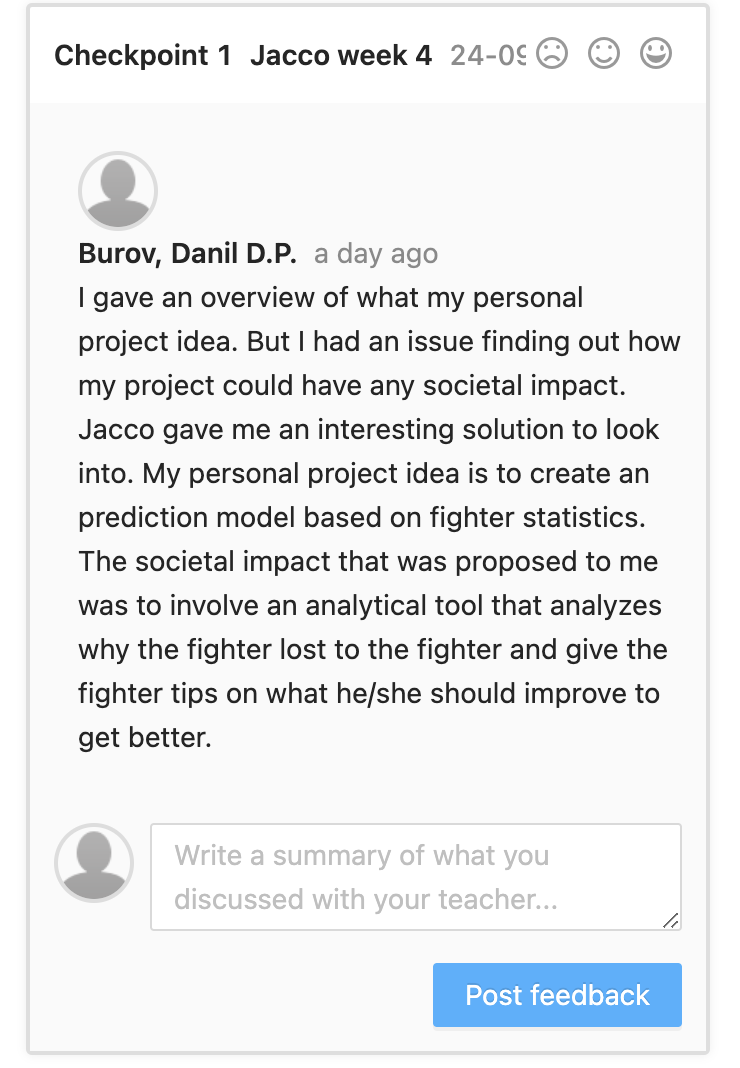
\includegraphics{images/Feedback_Societal_Impact.png}
  \caption{Feedback checkpoint for societal impact}
  \label{fig:appendix_image1}
\end{figure}

\end{document}
